% ESE580 Machine Perception - Structure from Motion Progress Report

\documentclass{article}
\usepackage{graphicx}
\usepackage{color}
\usepackage{listings}
\usepackage{fullpage}
\usepackage{amsmath}
\usepackage{placeins}

\definecolor{lightgray}{gray}{0.5}
\setlength{\parindent}{0pt}
\setcounter{secnumdepth}{0} %turn off section numbering
\begin{document}

\title{ESE580 Final Project: Structure from Motion}
\author{Joe Trovato}
\date{\today}
\maketitle
\setlength{\parindent}{10ex}

\section{Introduction}
\par
Structure from Motion involves a plethora of key steps. Each of these step refines the estimated camera positions and the 3D points being reconstructed from the images. I have implemented most of the components and I am working on a way to track matches through multiple images and the 3D structure. My nonlinear optimizations are also giving me trouble so I am attempting to complete the pipeline with the non-linear optimization steps. I realize this will give inaccurate results, but once the pipeline is in place, I believe I will have a better understanding and will be able to implement the non-linear optimizations. 

\section{Progress}

\subsection{RANSAC}
I have implemented RANSAC to robustly remove outliers from the matches provided to us. I found that there were very few outliers and that RANSAC selected most of the points as inlier after 100 iterations. 
\FloatBarrier

\begin{figure}[!h]
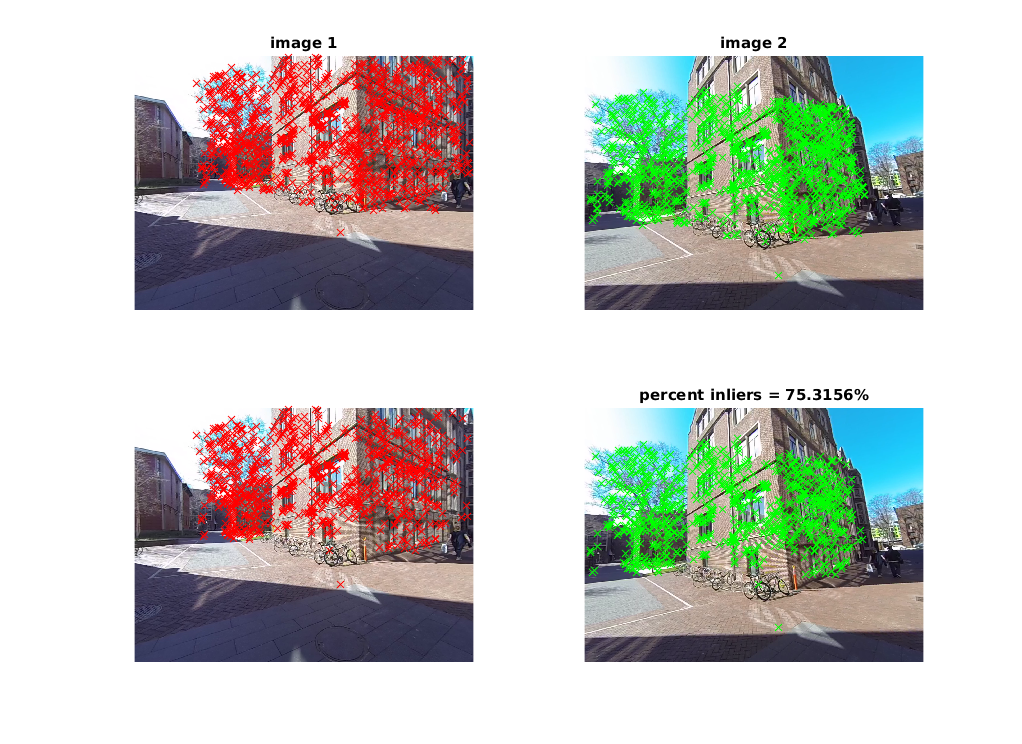
\includegraphics[width = \textwidth]{orig_and_ransac.png}
\centering
\caption{The original matches are shown in the top row of images. The inliers determined by RANSAC are int he bottom row.}
\end{figure}

\begin{figure}[!h]
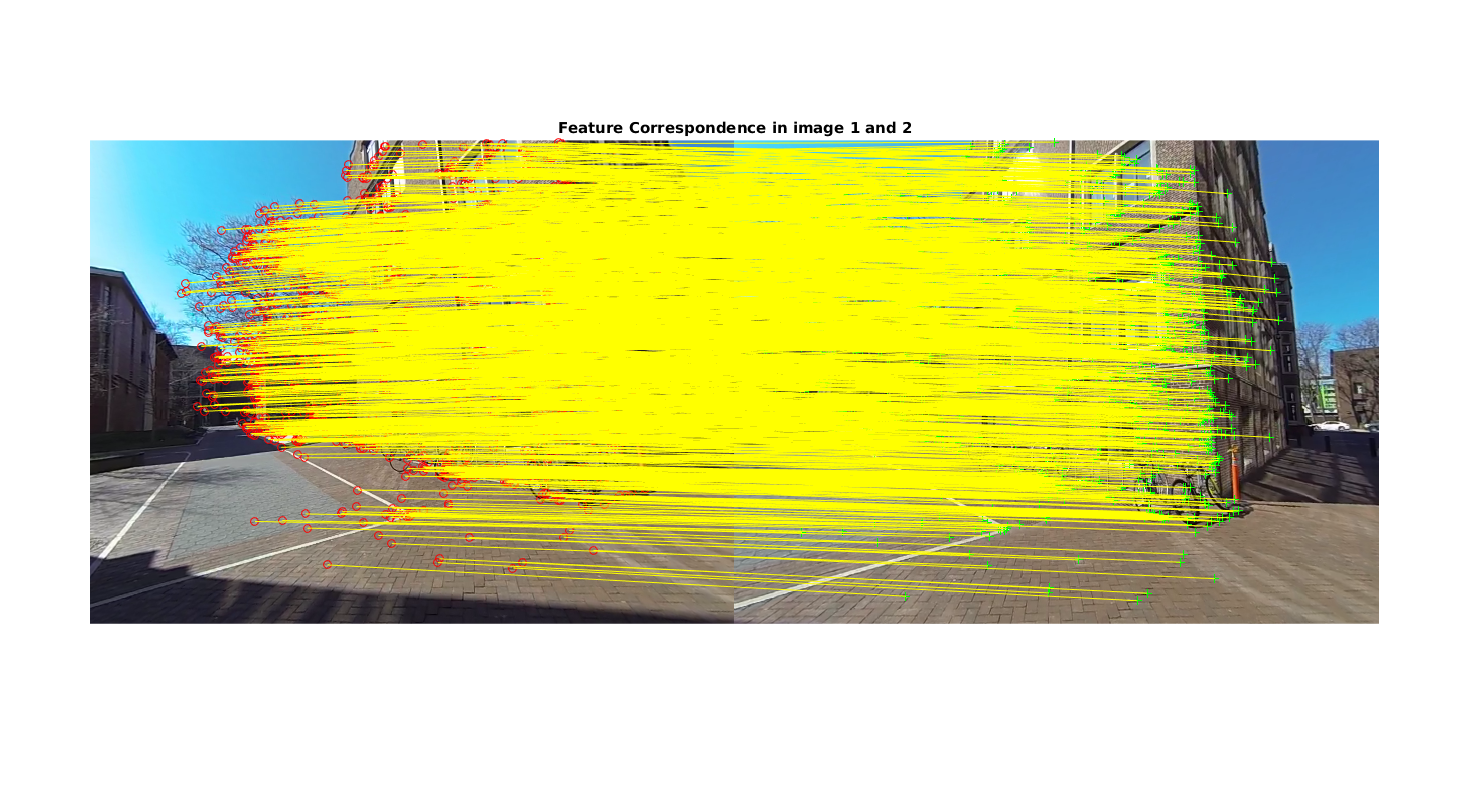
\includegraphics[width = \textwidth]{matches.png}
\centering
\caption{Matches shown with their exact correspondence in the second image. }
\end{figure}
\FloatBarrier
\subsection{Triangulation}
I have implemented the linear triangulation between two images and disambiguated the camera pose. The result is a 3D point cloud that looks like a building. I have not been able to get non-linear triangulation working, but believe it will improve the point cloud.
\FloatBarrier

\begin{figure}[!h]
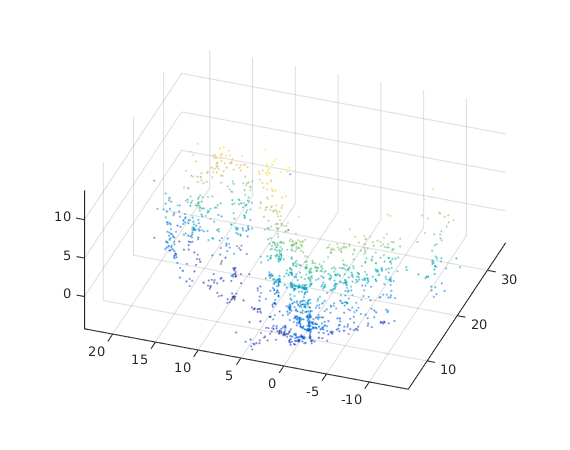
\includegraphics[width = \textwidth]{lin_tri.png}
\centering
\caption{View of the point cloud generated by linear triangulation from above the camera position}
\end{figure}

\begin{figure}[!h]
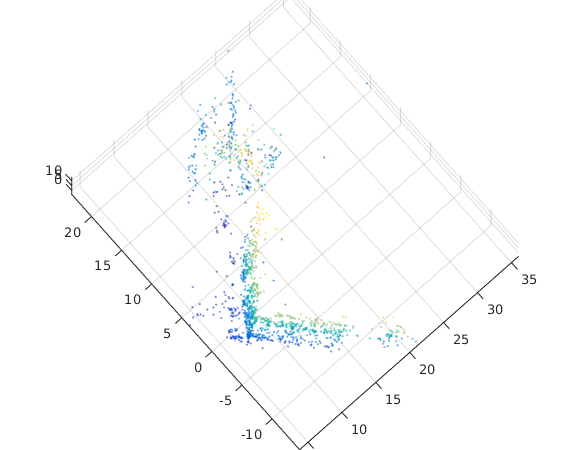
\includegraphics[width = \textwidth]{lin_tri_top.png}
\centering
\caption{View of the point cloud generated by linear triangulation from a bird's eye view}
\end{figure}

\FloatBarrier
\end{document}